% Segundo \cite{horn86robot}, todo triângulo equilátero tem os lados iguais. Já
% segundo \cite{shashua97photometric}, todo quadrado também tem.

% Veja que o pacote \verb|natbib| permite uma série de formas diferentes para
% fazer referências bibliográficas. O comando padrão, \verb|\cite|, realiza a
% citação comum vista no parágrafo anterior. Outros comandos permitem, por
% exemplo, citar somente o autor --- por exemplo, citar o trabalho de
% \citeauthor{samaras99coupled} --- ou colocar automaticamente a citação entre
% parênteses \citep{hougen93estimation, sato99illumination2, sato99illumination1,
% sato01stability}. Os comandos usados foram, respectivamente, \verb|\citeauthor|
% e \verb|\citep|. Veja a documentação do \verb|natbib| na Internet para conhecer
% outros comandos e exemplos de uso.

% Citações aleatórias para fazer com que as referências bibliográficas ocupem
% mais de uma página: \cite{bichsel92simple, dror01statistics, guisser92new}.


% \section{Motivação}

% \dummytxtb\dummytxta

% \subsection{Sub-motivação}


% \dummytxtc\dummytxtb

% \subsection{Mais uma sub-seção}

% \dummytxta\dummytxtc

% \subsubsection{Descendo mais um nível}

% \dummytxtb\dummytxta


% \chapter{Desenvolvimento}

% \dummytxtb\dummytxta\dummytxtc

% \begin{figure}[t]
%     \centering
%     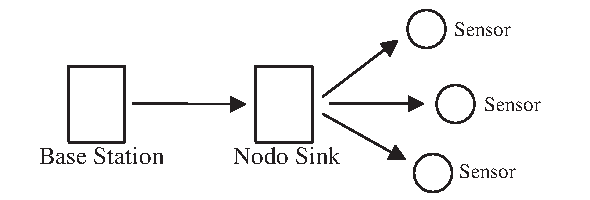
\includegraphics{img/exemplo}
%     \caption{Uma figura de exemplo.}
%     \label{fig:exemplo}
% \end{figure}

% \dummytxtb\dummytxta\dummytxtc\dummytxtb

% \begin{table}[t]
%     \caption{Uma tabela de exemplo.}
%     {\centering
%     \begin{tabular}{lcr} \toprule
%     \emph{Left-aligned} & \emph{Centered} & \emph{Right-aligned} \\ \midrule
%     Lorem ipsum & dolor sit & amet \\
%     consectetur adipisicing & elit, sed do eiusmod & tempor \\
%     incididunt ut & labore et dolore & magna aliqua. \\ \bottomrule
%     \end{tabular}\par
%     }
% \end{table}

% Este comando encapsula o conjunto de apêndices. A sua função é fazer com que
% a numeração dos apêndices seja feita com letras maiúsculas (A, B, C, etc.) e
% a palavra "Apêndice" anteceda as entradas no Sumário.
% \begin{appendices}

% % Para cada apêndice, um \chapter
% \chapter{Um apêndice}

% \dummytxta
% \dummytxtb
% \dummytxtc
% \dummytxta
% \dummytxtb

% \chapter{Outro apêndice}

% \dummytxta
% \dummytxtb
% \dummytxtc
% \dummytxta
% \dummytxtb

% % Fim dos apêndices (usar apenas depois do último apêndice)
% \end{appendices}


% % Este comando encapsula o conjunto de anexos. A sua função é fazer com que a
% % numeração dos anexos seja feita com letras maiúsculas (A, B, C, etc.) e a
% % palavra "Anexo" anteceda as entradas no Sumário.
% \begin{attachments}

% % Para cada anexo, um \chapter
% \chapter{Um anexo}

% \dummytxta
% \dummytxtb
% \dummytxtc
% \dummytxta
% \dummytxtb

% \chapter{Outro anexo}

% \dummytxta
% \dummytxtb

% % Fim dos anexos (usar apenas depois do último anexo)
% \end{attachments}

